\documentclass[12pt]{article}
 
 \usepackage{mathpazo}
 
\usepackage[brazil]{babel}                                 
\usepackage[T1]{fontenc} 
\usepackage[utf8]{inputenc}
 
\usepackage[margin=0.5in]{geometry}
\usepackage{amsmath,amsthm,amssymb}

%pacotes para fazer letra cursiva
\usepackage{mathrsfs}

%%necessario para alguns simbolos matematicos, como \quad
\usepackage{amssymb}

%legenda ao lado das figuras
\usepackage{sidecap}

\usepackage{hyperref}% add hypertext capabilities

\usepackage{subfigure}
\usepackage[pdftex]{graphicx}

%para nao ficar o retangulo em volta dos links, apenas muda a cor dos caracteres
\hypersetup{ colorlinks,
linkcolor=blue,
filecolor=blue,
urlcolor=blue,
citecolor=blue }

% altera a fonte nas legendas das figuras
\usepackage[font=small,format=plain,labelfont=bf,up,textfont=it,up]{caption}
 

\newenvironment{problem}[2][{\color{red}Problema}]{\begin{trivlist}
\item[\hskip \labelsep {\bfseries #1}\hskip \labelsep {\bfseries #2.}]}{\end{trivlist}}

\setlength{\parskip}{0,3em}  %altera o espaco entre dois paragrafos
\renewcommand{\baselinestretch}{1.1} %altera o espacamento entre as linhas
 
\begin{document}
 
\title{{\color{blue}Prova 3}}
\author{Prof. Paulo Freitas Gomes, Física 1}
 
\maketitle
 
\begin{problem}{{\color{red}1}}
\text{Centro de massa}\\
Uma mulher de 45 kg fica em pé em uma canoa de 60 kg e 5 m de comprimento (veja figura \ref{canoa}). Ela anda de um ponto a 1 metro de distância da extremidade até outro ponto a 1 metro da outra extremidade. Ignore a resistência da água na canoa. a) Qual o deslocamento da canoa durante o caminhar da moça? b) Qual a distância que a mulher percorreu em relação a água? c) Quem (ou o que) exerceu a força na canoa que a fez se mover?
\end{problem}

\begin{problem}{{\color{red}2}}
\text{Colisão Inelástica}\\
Duas massas idênticas são liberadas do repouso em uma superfície hemisférica de raio $R$ (veja figura \ref{cunha}). Despreze o atrito entre as massas e a superfície. a) Supondo uma colisão totalmente inelástica, qual a altura que as massas alcançam? b) E se a colisão for elástica, o que acontece?
\end{problem}


\begin{problem}{{\color{red}3}}
\text{Colisão em duas dimensões}\\
Em uma transportadora de carga, um carrinho aberto com massa de 50 kg roda da direita para a esquerda com velocidade escalar de 5 m/s (veja figura \ref{calha}). Despreze o atrito entre o carrinho e o piso. Um pacote de 15 kg desliza de cima para baixo por uma calha que está inclinada de 37 graus do plano horizontal e deixa o final da calha com velocidade de 3 m/s. O pacote cai dentro do carrinho e eles rodam juntos. Considerando que o final da calha está a uma altura de 4 m acima do fundo do carrinho, quais são a) a velocidade escalar do pacote pouco antes de cair dentro do carrinho e b) a velocidade escalar final do carrinho?
\end{problem}


\begin{problem}{{\color{red}4}}
\text{Colisão elástica com mola}\\
Um bloco de massa $m_1=$ 1.6 kg se move para a direita com uma velocidade de 4 m/s em uma superfície horizontal sem atrito. Ele colide com uma mola leve presa em um segundo bloco de massa $m_2=$ 2.1 kg inicialmente se movendo para a esquerda com velocidade de 2.5 m/s (veja figura \ref{blocos_molas}). A constante de mola é 600 N/m. a) Calcule a velocidade dos dois blocos após a colisão. b) Quando os blocos começam a comprimir a mola, eles perdem velocidade. Calcule a velocidade do bloco 2 durante a colisão no instante que o bloco 1 está se movendo para a direita com velocidade 3 m/s, como na figura \ref{bloco_mola_b}. c) Calcule a compressão da mola nesse instante. d) Suponha que a mola seja real (tendo uma certa massa). Explique se energia total é conservada ou não.
\end{problem}

\begin{problem}{{\color{red}5}}
\text{Salto em altura}\\
Na Olimpíada de 1968 o saltador Dick Fosbury introduziu uma nova técnica de salto em altura, a qual permitiu que o recorde mundial subisse cerca de 30 cm. Javier Sotomayor é o atual detentor do recorde mundial: 2.45 metros, marca obtida em 1993! Nesta técnica, o saltador passa sobre a barra com o rosto virado para cima enquanto arqueia suas costas (veja figura\footnote{{\scriptsize \url{http://www.athleticsweekly.com/iaaf-world-championships/world-championships-womens-high-jump-30993}.}} \ref{high_jump}). a) Considere o saltador como sendo uma barra uniforme e fina de comprimento $L$ e curvada sob um ângulo de $\theta =$ 90 graus (veja figura \ref{barra_curva}). Onde está o centro de massa da barra? Faça um desenho cuidadoso e indique a posição com boa aproximação. b) Por que esta técnica permite uma altura maior? c) Qual a relação da técnica de Fosbury com o famoso movimento de ballet chamado \textit{Grand Jeté}?. 
\end{problem}

\begin{figure}%[!h]
\centering
\subfigure{a)
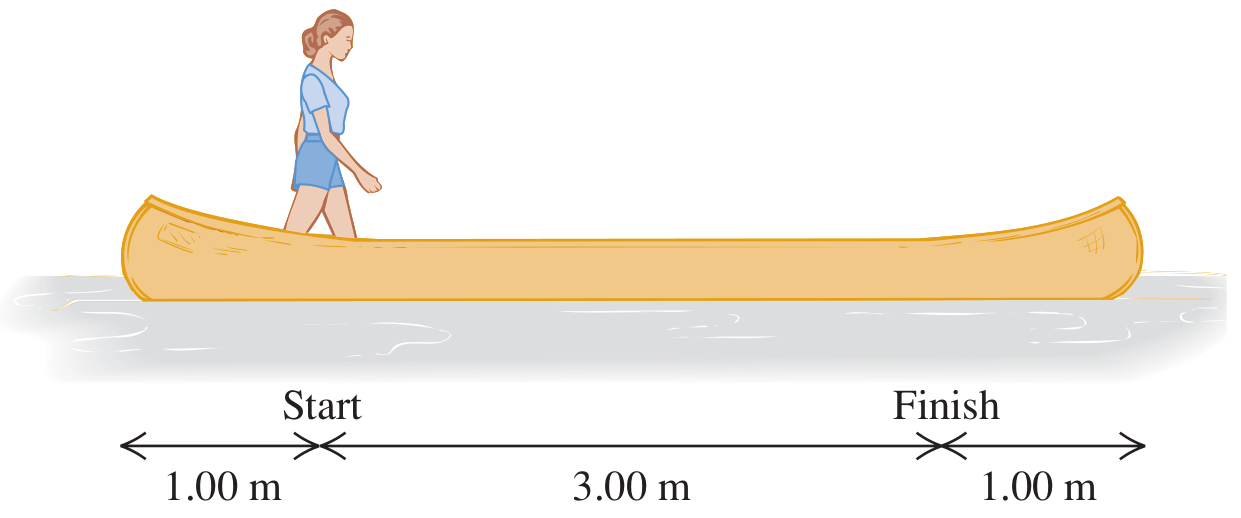
\includegraphics[width=5.4 in]{figuras/canoa.png}
\label{canoa}
}
\subfigure{b)
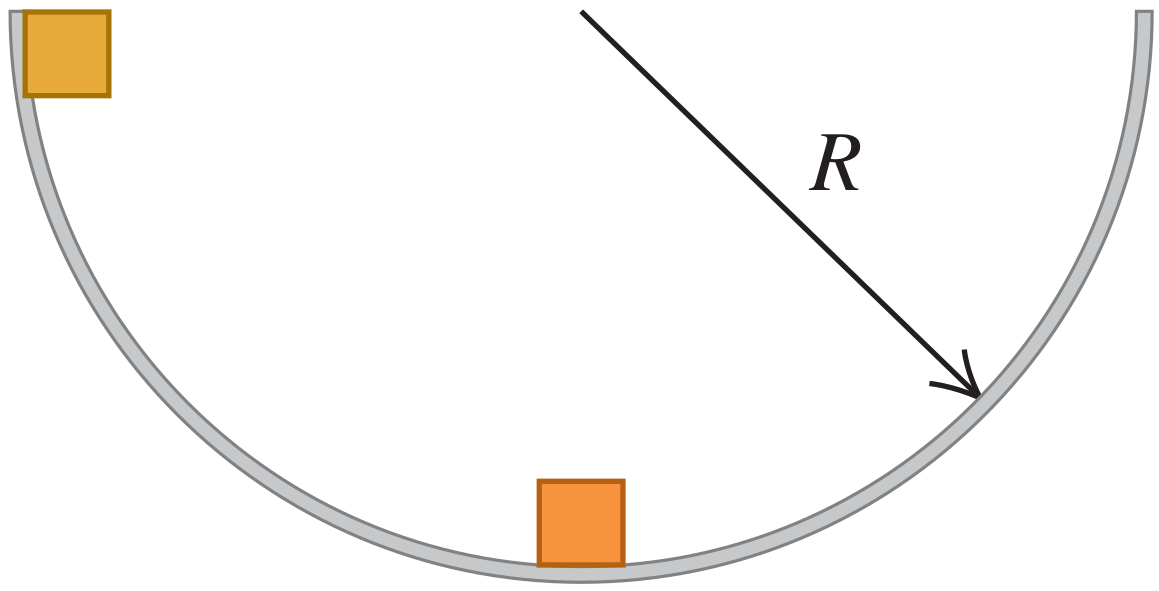
\includegraphics[width=2.5 in]{figuras/cunha.png}
\label{cunha} 
} 
\subfigure{c)
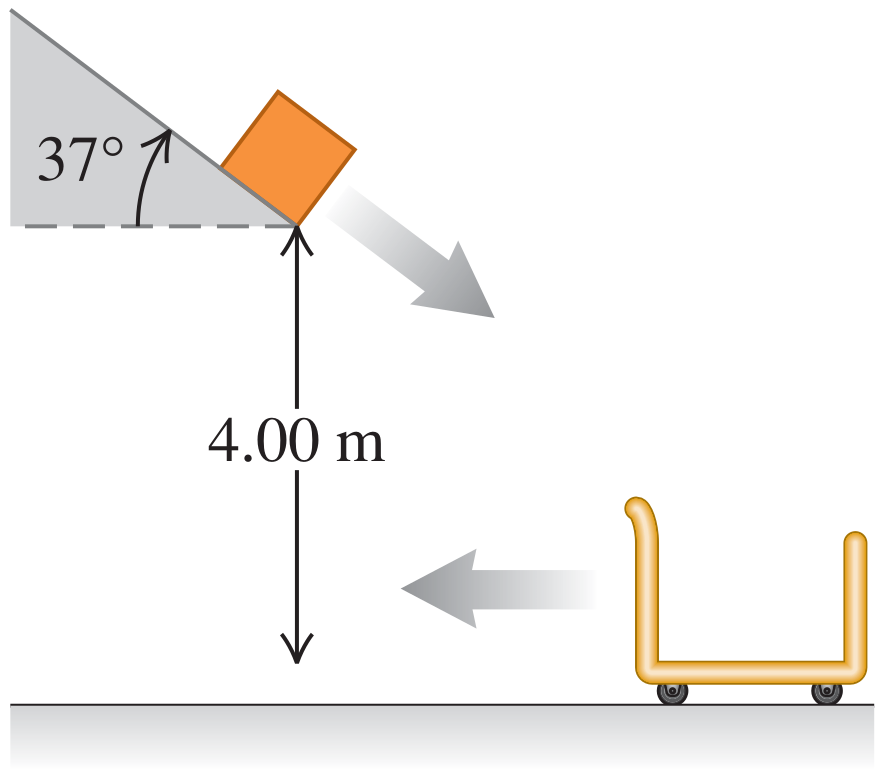
\includegraphics[width=2.3 in]{figuras/calha.png}
\label{calha}
}
\subfigure{d)
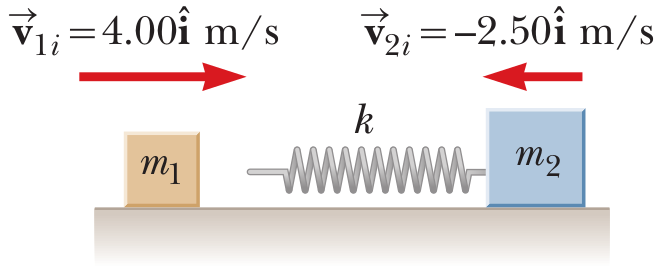
\includegraphics[width=3.4 in]{figuras/blocos_molas.png}
\label{blocos_molas}
} 
\subfigure{d)
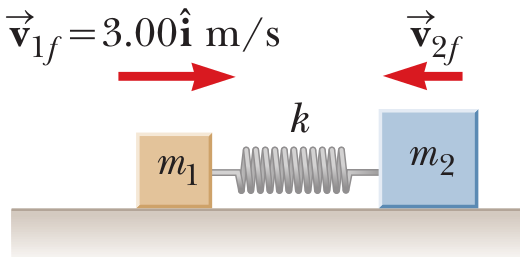
\includegraphics[width=2.8 in]{figuras/bloco_mola_b.png}
\label{bloco_mola_b}
} 
\caption{\subref{canoa} Problema 1. \subref{cunha} Problema 2. \subref{calha} Problema 3. \subref{blocos_molas} Problema 4. \subref{bloco_mola_b} Problema 4.}
\end{figure}


 \begin{figure}
 \centering
 \subfigure{a)
 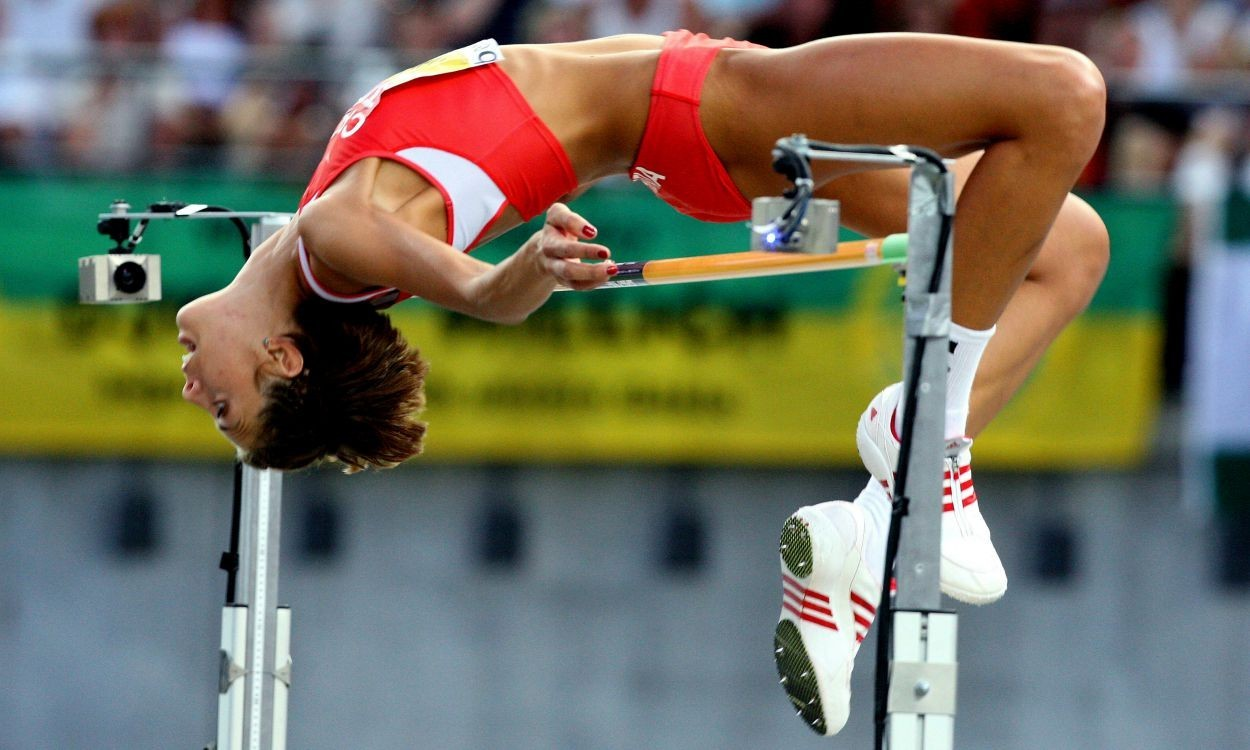
\includegraphics[width=3.8 in]{figuras/high_jump.jpg}
 \label{high_jump}
 }
 \subfigure{b)
 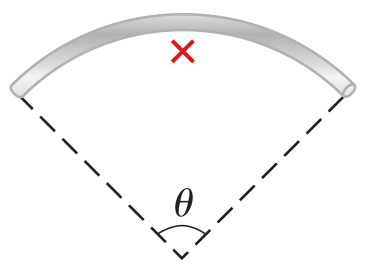
\includegraphics[width=2.2 in]{figuras/barra_curva.png}
 \label{barra_curva} 
 }
 \caption{Figuras referente ao problema 5. \subref{high_jump} Momento em que uma saltador passa sobre a barra. \subref{barra_curva} Barra uniforme curva fazendo um ângulo de 90 graus.}
 \end{figure}
 
 \begin{flushright}
\begin{small}
\textbf{Inspiração:}
{\color{blue}\textit{Você não pode ligar os pontos olhando pra frente, você só pode conectá-los olhando para o passado. Então, você tem que confiar que os pontos vão se ligar no seu futuro de alguma forma. Você tem que confiar em algo - seu instinto, destino, vida, carma, o que quer que seja. Porque acreditar que os pontos vão se ligar lá na frente vai lhe dar a confiança para seguir seu coração, mesmo quando ele lhe guiar para fora do caminho seguro e confortável. E isto fará toda a diferença.}}  \\
\textbf{Steve Jobs}
\end{small}
\end{flushright}

\newpage

{\color{red}\textbf{Gabarito}}

\begin{problem}{1}
a) Não há força externa então o centro de massa do sistema canoa $+$ mulher deve permanecer em repouso. Quando a mulher caminha sobre a canoa, sua posição muda. Para que o centro de massa do sistema continue na mesma posição a canoa deve se mover em sentido contrário. Seja a mulher o corpo A e a canoa o corpo B. Logo $m_A =$ 45 kg e $m_B=$ 60 kg e o comprimento da canoa é $L=$ 5 m. Vamos considerar a canoa como tendo toda sua massa localizada em seu centro de massa, que fica em seu centro geométrico. Seja o eixo $x$ apontando para a direita com a origem na extremidade esquerda da canoa. As posições iniciais da mulher e da canoa são: $x_{a1}=$ 1 m e $x_{b1}=L/2=$ 2.5 m. A posição do centro de massa antes é:
\begin{equation}
x_1 = \dfrac{m_A x_{a1} + m_B x_{b1}}{m_A + m_B}. \nonumber
\end{equation}
Depois que a mulher anda as novas posições são: $x_{a2} =x_{b2}+d$ com $d=$ 1.5 m (já que agora ela está a 1 m da extremidade direita da canoa) onde $x_{b2}$ é a nova posição do centro de massa da canoa. O centro de massa do sistema agora é:
\begin{equation}
x_2 = \dfrac{m_A x_{a2} + m_B x_{b2}}{m_A + m_B}. \nonumber
\end{equation}
Fazendo $x_1 = x_2$ temos:
\begin{equation}
m_A x_{a1} + m_B x_{b1} = m_A x_{a2} + m_B x_{b2}. \nonumber
\end{equation}
A única variável desconhecida é $x_{b2}$:
\begin{equation}
x_{b2} = \dfrac{m_A x_{a1} + m_B x_{b1} - m_A d}{m_A + m_B} = 1.21 \quad \text{m}. \nonumber
\end{equation}
O deslocamento da canoa é então {\color{red}$x_{b2} - x_{b1}= 1.21 - 2.5 = - 1.29$ m}.

\noindent
b) A mulher caminha 3 metros para a direita em relação a canoa que se desloca 1.29 metros para a esquerda. Logo a mulher caminha {\color{red}$3 - 1.29 = 1.71$ m} em relação a água para a direita.

\noindent
c) A canoa se move devido a força de contato com os pés da mulher: a mulher empurra a canoa para trás enquanto a canoa empurra de volta a mulher para frente. Como essas forças são internas, não há deslocamento efetivo (da mesma forma que não há quando andamos de carro).
\end{problem}

\begin{center}
\noindent\rule{13cm}{0.5pt}
\end{center}

\begin{problem}{2}
a) Quando as duas massas após a colisão sobem a rampa elas ganham energia potencial gravitacional que deve ser igual a energia cinética imediatamente após a colisão: $2mgy = \frac{1}{2}2mv_d^2$ onde $m$ é a massa de cada partícula, $y$ é a altura desejada e $v_d$ é a velocidade das massas após a colisão. Para achar $v_d$ aplicamos a conservação de momento antes e depois da colisão: $mv_a = 2mv_d$, o que implica em $v_d = v_a/2$. Para achar $v_a$ devemos lembrar que a energia cinética que a massa adquiriu vem da energia potencial gravitacional: $mgR = \frac{1}{2}mv_a$, logo $v_a = \sqrt{2gR}$. Substituindo tudo de volta temos:
\begin{equation}
y = \dfrac{v_d^2}{2g} = \dfrac{v_a^2}{8g} = \dfrac{2gR}{8g} = {\color{red}\dfrac{R}{4}}. \nonumber  
\end{equation}

\noindent
b) Se a colisão for elástica teremos o chamado pêndulo de Newton. Após a colisão o bloco da esquerda fica parado e o da direita se desloca com a mesma velocidade, subindo até uma altura idêntica a altura inicial do bloco da esquerda. Depois ele retorna e colide com o bloco da esquerda que sobe e desce, colide com o da direita que sobe e desce... e assim sucessivamente. O pêndulo de Newton consiste do mesmo fenômeno, porém com mais de uma massa e sendo todas elas suspensas.

\end{problem}


\begin{center}
\noindent\rule{13cm}{0.5pt}
\end{center}

\begin{problem}{3}
a) Vamos usar a conservação da energia mecânica total: $K_1+U_1 = K_2+U_2$. Instante antes: momento em que o pacote deixa a calha com $v_1=3$ m/s e $h=4$ m. Instante depois: momento imediatamente antes do pacote atingir o carrinho. Vamos assumir o referencial de altura no carrinho de forma que $U_2=0$. Logo:
\begin{equation}
\frac{1}{2}mv_1^2 + mgh = \frac{1}{2}mv_2^2. \nonumber 
\end{equation}
A quantidade desejada é $v_2$:
{\color{red}
\begin{equation}
v_2 = \sqrt{v_1^2 + 2gh} = \sqrt{3^2 + 2\cdot 9.8 \cdot 4} = 9.35 \quad \text{m/s}. \nonumber  
\end{equation}}

\noindent
b) Quando o pacote atinge o carrinho o momento é conservado apenas na horizontal (pois na vertical há uma força normal do chão no carrinho). Seja a direção $+x$ para a direita, o pacote designado por A e o carrinho por B. Como a colisão é totalmente inelástica, a conservação do momento nos dá:
\begin{equation}
m_a v_{a1} + m_bv_{b1} = (m_a+m_b)v_f, \nonumber
\end{equation}
onde $v_{b1} = -5$ m/s e $v_{a1} = v_1 \cos \theta$ é a velocidade horizontal do pacote (constante durante a queda). O ângulo que o vetor velocidade faz com a horizontal é $\theta = 37$ graus. A quantidade desejada é $v_f$:
{\color{red}
\begin{equation}
v_f = \dfrac{m_a v_{a1} + m_bv_{b1}}{m_a+m_b} = \dfrac{15 \cdot 3 \cdot \cos (37) - 50 \cdot 5}{15+50} = -3.29 \quad \text{m/s}.  \nonumber
\end{equation}} 
 
 

\end{problem}

\begin{center}
\noindent\rule{13cm}{0.5pt}
\end{center}

\begin{problem}{4} 
a) As velocidades iniciais são: $v_{1i}=4$ m/s e $v_{2i}=-2,5$ m/s. Como não há forças externas o momento é conservado:
\begin{equation}
m_1 v_{1i} + m_2 v_{2i} = m_1 v_{1f} + m_2 v_{2f}. \label{consermomentpro4}
\end{equation}
Como a colisão é elástica a energia cinética também é conservada:
\begin{equation}
\frac{1}{2} m_1 v_{1i}^2 + \frac{1}{2} m_2 v_{2i}^2 = \frac{1}{2} m_1 v_{1f}^2 + \frac{1}{2} m_2 v_{2f}^2. \nonumber
\end{equation}
Temos então duas equações e duas incógnitas: $v_{1f}$ e $v_{2f}$, de modo que é possível resolver o problema. Porém, é trabalhoso. Uma forma mais simples é usar a conservação da velocidade relativa:
\begin{equation}
v_{1i} -v_{2i} =  -(v_{1f} - v_{2f}). \label{sljconver53}
\end{equation}
no lugar da conservação de energia cinética. Multiplicando a Eq. \ref{sljconver53} por $m_1$ e somando com a Eq. \ref{consermomentpro4} temos:
\begin{equation}
2m_1 v_{1i} + (m_2-m_1)v_{2i} = (m_1+m_2)v_{2f}. \nonumber
\end{equation}
Logo:
{\color{red}
\begin{equation}
v_{2f} = \dfrac{2m_1 v_{1i} + (m_2-m_1)v_{2i}}{m_1+m_2} = 3,12 \quad \text{m/s}. \nonumber
\end{equation}}

Agora voltamos na conservação da velocidade relativa (Eq. \ref{sljconver53}) para achar $v_{1f}$:
{\color{red}
\begin{equation}
v_{1f} = v_{2f} - v_{1i} + v_{2i} = 3,12 - 4,0 + (-2,5) = -3,38 \quad \text{m/s}. \nonumber
\end{equation}}

\noindent
b) Para achar $v_{2f}$ aplicamos novamente a conservação do momento mas agora considerando $v_{1f}=3$ m/s. Isolando temos $v_{2f}$ da Eq. \ref{consermomentpro4}, temos:
{\color{red}
\begin{equation} 
v_{2f} = \dfrac{m_1 v_{1i} + m_2 v_{2i} - m_1 v_{1f}}{m_2}=-1,74 \quad \text{m/s}. \nonumber
\end{equation}}
O sinal negativo indica que o bloco 2 ainda está se movendo para a esquerda. O fato da mola estar comprimida não influi na conservação do momento, já que estamos assumindo uma mola sem massa (leve, como dita no enunciado).

\noindent
c) Vamos usar a conservação da energia cinética. Escolhemos como momento antes a situação inicial antes da colisão, com energia total:
\begin{equation}
E_i = \frac{1}{2} m_1 v_{1i}^2 + \frac{1}{2} m_2 v_{2i}^2. \nonumber
\end{equation}
Já no instante em questão (o mesmo do item b) a mola guarda energia potencial elástica. A energia total nesse instante é:
\begin{equation}
E_f = \frac{1}{2} m_1 v_{1f}^2 + \frac{1}{2} m_2 v_{2f}^2 + \frac{1}{2}kx^2, \nonumber
\end{equation}
onde $v_{1f}$ e $v_{2f}$ são os mesmos do item b). Fazendo $E_i=E_f$ e isolando $x$ temos:
{\color{red}
\begin{equation}
x = \sqrt{ \dfrac{1}{k} \left[  m_1 ( v_{1i}^2 - v_{1f}^2)  + m_2 (v_{2i}^2 - v_{2f}^2) \right] } = 0,173 \quad \text{m}. \nonumber
\end{equation}}
\end{problem}

\noindent
d) Sendo a mola real a energia mecânica total não será conservada pois parte dela irá se transformar em calor quando a mola for comprimida. Além disso a conservação do momento usada no item b) deve incluir o termo de momento da mola (que é bem trabalhoso de calcular!!).

\begin{center}
\noindent\rule{13cm}{0.5pt}
\end{center}

\begin{SCfigure}
\centering
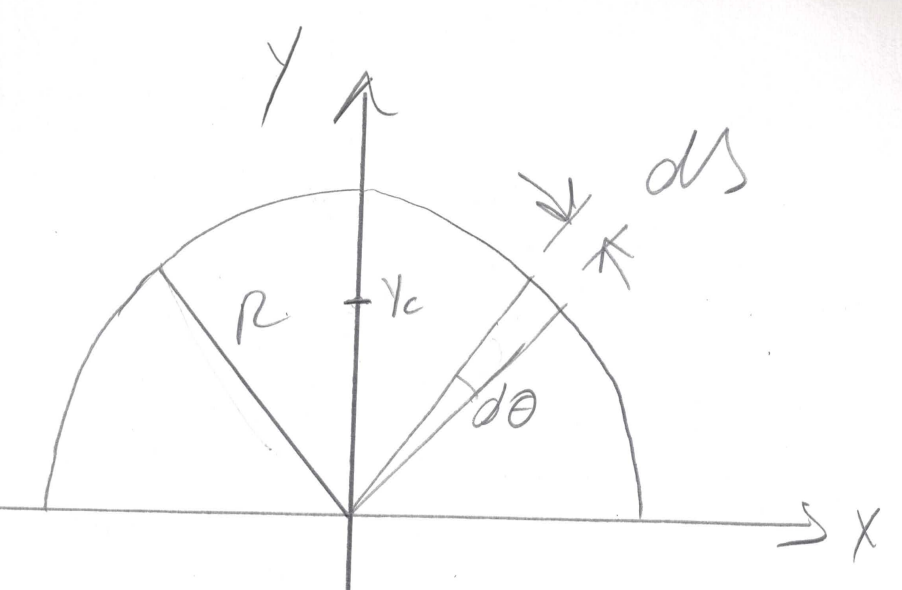
\includegraphics[width=3.5 in]{figuras/barra_geometria.png}
\caption{Figura referente a solução do item 5a).}
\label{barra_geometria}
\end{SCfigure}

\begin{problem}{5}
a) A definição das coordenadas do centro de massa são:
\begin{equation}
x_c = \dfrac{\sum_i m_i x_i}{\sum_i m_i}, \qquad y_c = \dfrac{\sum_i m_i y_i}{\sum_i m_i}. \nonumber
\end{equation}
Considere a geometria no plano $xy$ como mostrado na figura \ref{barra_geometria}. Pela simetria temos que $x_c = 0$ já que há uma quantidade igual de massa em ambos os lados do eixo $y$. Para calcular $y_c$ transformamos o somatório em uma integral já que a barra é uma distribuição contínua de massa:
\begin{equation}
y_c = \dfrac{1}{M} \int y dm, \nonumber
\end{equation}
onde $M=\sum_i m_i$ é a massa da barra e $dm$ é o elemento infinitesimal de massa. A densidade linear de massa é $\lambda = M/L$ onde $L=\pi R$ é o seu comprimento e $R$ o raio. Supondo uma distribuição uniforme de massa podemos escrever $\lambda = dm/ds$ onde $ds$ é o elemento de comprimento. Porém da definição de radiano e olhando a figura \ref{barra_geometria} temos que $ds = R d\theta$. Além disso temos também que $y=R\sin \theta$. Usando tudo isso:
\begin{eqnarray}
y_c &=& \dfrac{R^2 \lambda}{M} \int_0^{\pi}  \sin \theta  d\theta = - \dfrac{R^2 \lambda}{M} \cos \theta \bigg\rvert_0^{\pi} = 2 \dfrac{R^2 \lambda}{M} = \dfrac{R^2 \lambda}{\pi R \lambda}  \nonumber \\
 &=& {\color{red} \dfrac{2}{\pi}R \sim 0.64 R}. \nonumber
\end{eqnarray}
A integral é de 0 a $\pi$ pois engloba a metade do círculo. A posição $y_c$ está indicada na figura \ref{barra_geometria}.

\noindent
b) Esta técnica faz com que o centro de massa do corpo fique abaixo do mesmo. O impulso que o atleta faz para saltar é proporcional a altura do centro de massa. Assim ele consegue uma altura maior com o mesmo esforço já que seu corpo fica acima do centro de massa.

\noindent
c) O mesmo princípio é aplicado pelas Bailarinas no movimento Grand Jeté. A diferença é que agora as bailarinas moldam o corpo para que o mesmo fique abaixo do centro de massa. O objetivo é que o corpo se propague em uma linha reta. Como o centro de massa faz uma trajetória parabólica (lançamento oblíquo) a bailarina se movimenta para que o corpo não siga essa trajetória.
\end{problem}






\end{document}
